\id{ҒТАМР 20.23.25}

\begin{articleheader}
\sectionwithauthors{Н.Боранбаева, Б.Оразбаев, Л.Рзаева, Ж.Карабаев, Б.Серимбетов}{КАТАЛИТКАЛЫҚ КРЕКИНГ ҚОНДЫРҒЫСЫНАН ӨНІМНІҢ ШЫҒУЫН PYTHON
БАҒДАРЛАМАЛЫҚ ОРТАСЫН ҚОЛДАНУ АРҚЫЛЫ АНЫҚТАУ}

{\bfseries \textsuperscript{1}Н.Боранбаева,
\textsuperscript{1}Б.Оразбаев\textsuperscript{\envelope },
\textsuperscript{2}Л.Рзаева, \textsuperscript{3}Ж.Карабаев,
\textsuperscript{4}Б.Серимбетов}
\end{articleheader}

\begin{affiliation}
\textsuperscript{1}Л.Н.Гумилев атындағы Еуразия Ұлттық Университеті,
Астана, Қазақстан,

\textsuperscript{2}Astana IT University, Астана қ., Қазақстан,

\textsuperscript{3}Auezov University, Шымкент қ., Қазақстан,

\textsuperscript{4} Қ.Құлажанов атындағы Қазақ технология және бизнес
университеті, Астана, Қазақстан

\raggedright {\bfseries \textsuperscript{\envelope }}Корреспондент-автор: \href{mailto:batyr_o@mail.ru}{\nolinkurl{batyr\_o@mail.ru}}
\end{affiliation}

Мақалада Python бағдарламалық ортасында регрессия әдістерін қолдану
арқылы каталитикалық крекинг қондырғысынан өнімнің шығуын анықтау
тапсырмасы қарастырылады. Каталитикалық крекинг мұнай өндірудің негізгі
процесі болғандықтан, өнімнің шығуын нақты болжау технологиялық
параметрлерді оңтайландыру және өнімнің тиімділігін арттыру үшін өте
маңызды. Сараптама үшін Шымкент мұнай өндіру зауытының статистикалық
мәліметтері қолданылды, бұл ұсынылған әдісті нақты өндіріс шарттарында
қолдану мүмкіндігін көрсетеді. Мақалада реактордағы және регенератордағы
температура, қысым, шикізат тығыздығы және катализатор шығыны сияқты әр
түрлі технологиялық параметрлердің әсер етуін талдау нәтижесінде
модельдерді жасап шығару әдістемесі қарастырылған. Pandas, Scikit-learn
және Matplotlib сияқты Python мәліметтерді талдау инструменттері мен
кітапханаларын қолдану толық талдау жасап, нәтижелерін визуализациялауға
мүмкіндік береді. Модельдің сапасын бағалау детерминациялау коэфициенті
(R\textsuperscript{2}) және қалдық қателерді талдау арқылы жүргізіледі.
Алынған нәтижелер моделдің жоғарғы дәлдігі мен ұсынылған тәсілдің
өндірістегі мұнай өндіру процестерін болжау және оңтайландыру
мүмкіндігін дәлелдейді. Сондай-ақ, ұсынылған тәсілді мұнай өңдеу
процестерін оңтайландыру, технологиялық шешімдерді жақсарту және
мұнай-химия саласындағы өндірістердің жалпы экономикалық тиімділігін
арттыру үшін сәтті қолдануға болатындығы атап өтілді.

{\bfseries Түйін сөздер}: модельдеу, каталитикалық крекинг, python,
детерминациялау коэффициенті, айқын емес логика, компьютерлік модельдеу,
оңтайландыру, каталитикалық крекинг қондырғысы.

\begin{articleheader}
{\bfseries ОПРЕДЕЛЕНИЕ ВЫХОДА ПРОДУКТА ИЗ УСТАНОВКИ КАТАЛИТИЧЕСКОГО
КРЕКИНГА ИСПОЛЬЗОВАНИЕМ ПРОГРАМНОЙ СРЕДЫ PYTHON}

{\bfseries \textsuperscript{1}Н.Боранбаева,
\textsuperscript{1}Б.Оразбаев\textsuperscript{\envelope },
\textsuperscript{2}Л.Рзаева, \textsuperscript{3}Ж.Карабаев,
\textsuperscript{4}Б.Серимбетов}
\end{articleheader}

\begin{affiliation}
\textsuperscript{1}Евразийский Национальный Университет им.
Л.Н.Гумилева, г.Астана, Казахстан,

\textsuperscript{2}Astana IT University, г. Астана, Казахстан,

\textsuperscript{3}Auezov University, г. Шымкент, Казахстан,

\textsuperscript{4}Казахский университет технологии и бизнеса
им.К.Кулажанова,

е-mail: \href{mailto:batyr_o@mail.ru}{\nolinkurl{batyr\_o@mail.ru}}
\end{affiliation}

В данной статье рассматривается задача определение выхода продукта из
установки каталитического крекинга с использованием методов регрессии в
программной среде Python. Каталитический крекинг является одним из
ключевых процессов в нефтепереработке, и точное прогнозирование выхода
продукта имеет важное значение для оптимизации технологических
параметров и повышения эффективности производства. Для анализа
использованы статистические данные Шымкентского нефтеперерабатывающего
завода, что позволяет применить предложенные методы к реальным
производственным условиям. В работе представлены методология разработки
модели на основе анализа влияния различных технологических параметров,
таких как температура, давление, плотность сырья и расход катализатора.
Применение инструментов анализа данных и библиотек Python, таких как
Pandas, Scikit-learn и Matplotlib, позволяет провести детальный анализ и
визуализацию результатов. Оценка качества модели производится с помощью
коэффициента детерминации (R\textsuperscript{2}) и анализа остаточных
ошибок. Полученные результаты демонстрируют высокую точность модели и
подтверждают возможность использования предложенного подхода для
прогнозирования и оптимизации процессов нефтепереработки в промышленной
практике\emph{.} Также подчеркивается, что предложенный подход может
быть успешно применен для оптимизации процессов нефтепереработки,
улучшения технологических решений и повышения общей экономической
эффективности производств в нефтехимической отрасли.

{\bfseries Ключевые слова:} моделирование, каталитический крекинг, python,
коэффициент детерминации, нечеткая логика, компьютерное моделирование,
оптимизация, установка каталитического крекинга.

\begin{articleheader}
{\bfseries DETERMINATION OF PRODUCT YIELD FROM A CATALYTIC CRACKING UNIT
USING THE PYTHON PROGRAMMING ENVIRONMENT}

{\bfseries \textsuperscript{1}N.Boranbayeva,
\textsuperscript{1}B.Orazbayev\textsuperscript{\envelope },
\textsuperscript{2}L.Rzayeva, \textsuperscript{3}Zh.Karabayev,
\textsuperscript{4}B.Serimbetov}
\end{articleheader}

\begin{affiliation}
\textsuperscript{1} L. N. Gumilyov Eurasian National University, Astana,
Kazakhstan,

\textsuperscript{2}Astana IT University, г. Астана, Kazakhstan,

\textsuperscript{3}Auezov University, Shymkent, Kazakhstan,

\textsuperscript{4}K. Kulazhanov Kazakh University of Technology and
Business, Astana, Kazakhstan,

е-mail: \href{mailto:batyr_o@mail.ru}{\nolinkurl{batyr\_o@mail.ru}}
\end{affiliation}

This article addresses the task of forecasting product yield from a
catalytic cracking unit using regression methods within the Python
programming environment. Catalytic cracking is one of the key processes
in oil refining, and accurate product yield forecasting is crucial for
optimizing technological parameters and improving production efficiency.
Statistical data from the Shymkent Oil Refinery were used for the
analysis, which allows us to apply the proposed methods to real
production conditions. The paper presents a model development
methodology that analyzes various technological parameters, such as
temperature, pressure, feedstock density, and catalyst consumption.
Using data analysis tools and Python libraries, such as Pandas,
Scikit-learn, and Matplotlib, enables detailed analysis and
visualization of results. The model' s quality is
assessed using the coefficient of determination (R\textsuperscript{2})
and residual error analysis. The results obtained demonstrate the high
accuracy of the model and confirm the feasibility of using the proposed
approach for forecasting and optimizing oil refining processes in
industrial practice. Against the background of the growing relevance of
issues related to the diagnosis of brain stroke, modern research in the
field of medical diagnostics is trying to use advanced deep learning
methods to improve the detection of this serious disease. It is also
emphasized that the proposed approach can be successfully applied to
optimize refining processes, improve technological solutions and
increase the overall economic efficiency of production in the
petrochemical industry.

{\bfseries Keywords:} modeling, catalytic cracking, Python, coefficient of
determination, fuzzy logic, computer modeling, optimization, unit of
catalytic cracking.

\begin{multicols}{2}
{\bfseries Кіріспе.} Каталитикалық крекинг жоғары октанды бензиндер мен
басқа да жеңіл мұнай өнімдерін өндіруде шешуші рөл атқаратын мұнай
өңдеудегі маңызды процестердің бірі болып табылады. Бұл процестің
тиімділігі температура, қысым, шикізаттың тығыздығы және катализатордың
шығыны сияқты көптеген технологиялық параметрлерге тікелей байланысты.
Каталитикалық крекинг қондырғыларының жұмысын оңтайландыру және олардың
өнімділігін арттыру үшін технологиялық параметрлер туралы мәліметтер
негізінде өнімнің шығуын дәл болжау қажет. Деректерді талдау мен
машиналық оқытудың заманауи әдістері өндіріс процестерін едәуір жақсарта
алатын болжамды модельдерді құрудың қуатты құралдарын ұсынады. Атап
айтқанда, регрессиялық талдау машиналық оқытудың негізгі әдістерінің
бірі ретінде айнымалылар арасындағы байланысты талдау және әртүрлі
көрсеткіштерді болжау үшін кеңінен қолданылады.

Бұл мақалада Python бағдарламалық жасақтамасында жүзеге асырылған
регрессия әдістерін қолдана отырып, каталитикалық крекинг қондырғысынан
өнімнің шығуын болжау тәсілі ұсынылады. Python Pandas, Scikit-learn және
Matplotlib сияқты қуатты деректерді талдау және визуализация
кітапханаларының арқасында мұндай модельдерді өнеркәсіптік тәжірибеге
енгізу және жасақтау үшін таңдаулы құралға айналуда.

Бұл жұмыстың мақсаты болжау моделін әзірлеу және бағалау болып табылады,
ол өнімнің шығуын жоғары дәлдікпен болжап қана қоймай, сонымен қатар
нақты жағдайларда технологиялық процестерді одан әрі оңтайландыру үшін
осы болжамдарды қолдануға мүмкіндік береді. Мақалада параметрлерді
таңдаудан бастап болжау сапасын бағалауға дейінгі модельді әзірлеудің
барлық кезеңдері қарастырылады, сонымен қатар ұсынылған тәсілдің
тиімділігін растайтын нәтижелер талқыланады. Өнімнің каталитикалық
крекинг қондырғысынан шығуын болжау күрделі міндет болып табылады, ол
шикізаттың құрамы, процесс шарттары және катализатордың сипаттамалары
сияқты көптеген факторларды ескеруді талап етеді. Соңғы жылдары
мұнай-химия саласындағы зерттеушілер мен тәжірибешілер болжау дәлдігін
жақсарту және процесті оңтайландыру үшін деректерді талдау және
машиналық оқыту әдістеріне көбірек бет бұруда.

Регрессия-химиялық процестерді болжауда ең көп қолданылатын әдістердің
бірі. {[}1{]} жұмыста регрессиялық модельдер айнымалылар арасындағы
тәуелділікті талдаудың негізгі мүмкіндіктерін ұсынады. Зерттеулер
көрсеткендей, регрессиялық модельдер қарапайымдылығына қарамастан,
әсіресе деректерді алдын ала талдау және негізгі трендтерді анықтау
жағдайында күрделі тәсілдер үшін жақсы бастама бола алады, {[}2{]}.
Python бағдарламалық ортасының Pandas, NumPy және scikit-learn сияқты
қуатты кітапханалары мен құрылымдарының арқасында деректерді талдаудың
танымал құралына айналды. Бірқатар жұмыстар {[}3{]} бұл құралдар
регрессиялық модельдерді құру және бағалау процесін едәуір
жеңілдететінін атап өтті. Python сонымен қатар деректерді
визуализациялау және модельдеу үшін ыңғайлы құралдарды ұсынады, бұл оны
мұнай-химия практиктері үшін ерекше құнды етеді. Каталитикалық крекинг
саласындағы заманауи зерттеулер көбінесе нейрондық желілер сияқты
күрделі машиналық оқыту әдістерін қолдануды қамтиды {[}4{]}. Бұл әдістер
үлкен көлемдегі деректермен және күрделі тәуелділіктермен жұмыс
істегенде жоғары тиімділікті көрсетеді. Алайда, {[}5{]} атап өткендей,
мұндай әдістерді өнеркәсіптік тәжірибеге біріктіру айтарлықтай есептеу
ресурстарын және процестерді терең түсінуді қажет етеді. Қосымша
зерттеуді қажет ететін маңызды аспектілер - болжамдардың дәлдігі және
нәтижелерді түсіндіру. {[}6{]} ғылыми жұмыста атап өткендей,
қолданыстағы модельдер өзгеретін процестер жағдайында қайта оқыту және
дәлдіктің жеткіліксіздігімен жиі ұшырасады. Перспективалық бағыттарға
сызықтық регрессия элементтері мен машиналық оқытудың күрделі
алгоритмдерін біріктіретін гибридті модельдерді дамыту, сондай-ақ
деректерді жинау және алдын ала өңдеу әдістерін жақсарту кіреді {[}7{]}.

Әртүрлі дереккөздерді талдау нәтижелері каталитикалық крекинг қондырғысы
сияқты күрделі айқын емес сипатталған химиялық-технологиялық жүйелерді
басқару, модельдеу мәселелерінің жеткіліксіз зерттелгендігін көрсетеді.
Осыған байланысты модельдерді әзірлеу, оңтайландыру мәселелерін зерттеу,
күрделі айқын емес химиялық-технологиялық жүйелерді басқару үшін шешім
қабылдау тапсырмасын қалыптастыру заманауи ғылымның өзекті міндеті болып
қала береді. Математикалық модельдерді әзірлеу принциптері мен әдістерін
талдау, шешім қабылдау және өнеркәсіптік объектілерді оңтайландыру
нәтижесінде ғылыми жұмыстарда лингвистикалық модельдерді әзірлеу және
олардың жұмыс режимдерін оңтайландыру мәселелері аз қамтылғандығы
анықталды. Жұмыстарда {[}8, 9{]} математикалық модельдерді әзірлеу және
бастапқы ақпараттың айқынсыздығымен сипатталатын технологиялық
объектілердің параметрлерін оңтайландыру тәсілдері зерттеліп, ұсынылды.
2000 жылдан бастап Р.А. Алиева, н. Р. Юсупбекова, Azeem M. F., Taskin
H., Osofisan P. B. сияқты авторлардың каталитикалық крекингті басқару
алгоритмдерінде айқын емес логика әдістерін қолдану арқылы жүзеге
асырылған бірқатар еңбектері жарық көрді. Бірақ күрделі объектілерді
модельдеу және оңтайландыру бойынша осы және басқа талданған жұмыстарда
объектінің кіріс және шығыс параметрлері айқын емес модельдерді әзірлеу
мәселелері толық зерттелмеген. Сонымен қатар, оңтайландыру мәселелерін
шешудің белгілі әдістерінде есептің қойылуы кезеңінде айқын емес есеп
мәселе нақты есептер жиынтығына айналады және одан әрі қолданыстағы
әдістермен шешіледі. Бұл тәсілде көбінесе бастапқы жиналған айқын емес
ақпараттың едәуір бөлігі жоғалады (білім, сарапшылардың тәжірибесі),
нәтижесінде алынған шешімдердің шындыққа сәйкестігі төмендейді {[}10{]}.

Әдебиеттерге шолу өнімнің каталитикалық крекинг қондырғысынан өнімнің
шығуын анықтауда Python және регрессия әдісін қолдану процестерді
талдауға және оңтайландыруға арналған қуатты құралдарды қамтамасыз
ететінін көрсетеді. Дегенмен, дәлірек және сенімді нәтижелерге қол
жеткізу үшін деректерді талдаудың дәстүрлі әдістерімен бірге заманауи
әдістерді де ескеру қажет.

{\bfseries Материалдар мен әдістер.} Бұл жұмыстың зерттеу нысаны Шымкент
мұнай өңдеу зауытының титулы 1000 RFCC ауыр қалдықтардың каталитикалық
крекинг қондырғысының реактор-регенератор блогы болып табылады.
Каталитикалық крекинг қондырғысы тікелей мазуттан каталитикалық крекинг
процесі арқылы автомобиль бензиндері мен сұйытылған көмірсутек
газдарының жоғары октанды компонентін алуға арналған. Каталитикалық
крекинг процесінің жүруіне әсер ететін негізгі факторлар шикізаттың
физика-химиялық сипаттамалары, катализатордың қасиеттері, реактордағы
қысым, реактордағы шикізат температурасы, реактордың температурасы,
катализатордың шығыны болып табылады. Каталитикалық крекинг
қондырғысынан бензиннің шығуы мен сапасы шикізаттың құрамына,
реактордағы температура мен қысымға, шикізаттың берілу жылдамдығына,
регенератордағы температураға, регенератор-реактор блогының жұмыс
режиміне, крекинг катализаторларының түріне және басқа параметрлерге
байланысты. Технологиялық режимдер алынатын өнімінің түріне байланысты
майлы газ, бензин немесе дизель фракциясы ретінде ерекшеленеді. Басқару
объектісінің техникалық регламенті негізінде процестің негізгі
технологиялық параметрлері анықталды: реактордың жоғарғы бөлігіндегі
қысым, реактордан шығатын реакция газдарының температурасы,
регенератордан шығатын газдардың температурасы. Әрі қарай, процеске әсер
ететін басқару объектісінің кіріс, шығыс, ауытқушы айнымалылары
анықталады. Реактор блогындағы технологиялық параметрлер процесс
режимінің оңтайлы қаттылығына қол жеткізу мақсатында реттеледі. Терең
оқыту технологияларының дамуы диагностиканың дәлдігі мен жеделдігін
жақсартудың жаңа перспективаларын ұсына отырып, осы процеске белсенді
әсер етеді.

Анықтамалық векторлық әдіс (SVM) және кездейсоқ ормандар сияқты
Машиналық оқыту әдістерінің пайда болуы диагностиканы жақсартудағы
маңызды қадам болды. Бұл тәсілдер медициналық кескіндерді талдау
процесін автоматтандыруға мүмкіндік береді, бірақ көбінесе күрделі үш
өлшемді деректер мен үлкен көлемдегі ақпаратты өңдеуде шектеулерге тап
болады.

Нейрондық желілердің архитектуралары, соның ішінде конволюциялық
нейрондық желілер (CNN) және қайталанатын нейрондық желілер (RNN)
деректердегі кеңістіктік және уақыттық тәуелділіктерді ескере отырып,
жоғары дәлдікті қамтамасыз етеді {[}11{]}.

Каталитикалық крекинг-мұнай өңдеуді тереңдетуге бағытталған негізгі
процесс. Процесс келесі технологиялық агрегаттарды қамтитын
каталитикалық крекинг қондырғысында жүреді: бу конденсациясы жүйесі,
реактор-регенератор блогы, түтін газын дымқыл тазарту блогы, шикізатты
дайындау және ректификациялау блогы, сіңіру және газ фракциялау блогы.
Реактор мен регенератор арасындағы сұйық катализатордың үздіксіз айналуы
каталитикалық крекинг процестерін үздіксіз режимде жүргізуге мүмкіндік
береді {[}12{]}.
\end{multicols}

\begin{figure}[H]
	\centering
	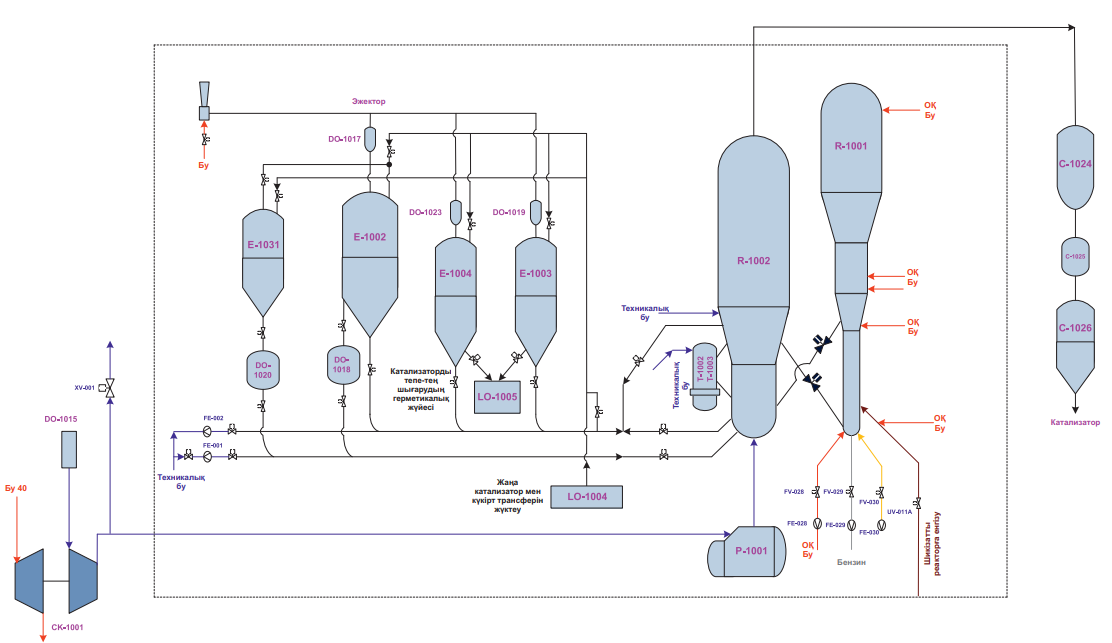
\includegraphics[width=0.8\textwidth]{media/ict/image86}
	\caption*{1 - сурет. RFCC каталитикалық крекинг қондырғысының реактор және
регенератор блогының технологиялық сызбасы}
\end{figure}

\begin{multicols}{2}
1-суретте RFCC 1000 титулды каталитикалық крекинг қондырғысының реактор
және регенератор блогының технологиялық схемасы көрсетілген {[}13{]}.
Қондырғының шикізаты - шикізатты араластыру контейнеріне берілетін
тікелей айдау мазуты немесе мазут қоспасы және тікелей айдау вакуумды
газойль фракциясының қоспасы. Араластыру контейнеріне шикізат сорғымен
реакторға беріледі, алдымен текше өнім ағындарының, жеңіл газойль
фракциясының (қажет болған жағдайда) және текше циркуляциялық суарудың
жылуы есебінен шикізат жылу алмастырғыштар блогында қызады. Реакторға
кіретін шикізаттың температурасы соңғы жылу алмастырғыштың айналма
жолындағы клапанмен реттеледі.

RFCC каталитикалық крекинг қондырғысында жұмыс жасайтын өндіріс
қызметкерлерінің, сарапшылардың сауалнамасынан алынған ақпарат реактор
блогының технологиялық жұмыс режимінің параметрлерінің өзгеру себептері
реакторға кіретін температураның өзгеруі, катализаторға жиналатын кокс
мөлшерінің өзгеруіне, сондай-ақ қоршаған ауа температурасының өзгеруіне
әкелетінін көрсетеді. Бұл өзгерістер регенератордың шығысындағы
катализаторының температурасына және реактордың кірісіндегі
катализатордың температурасына әсер етеді. Бұл каталитикалық крекинг
процесінің параметрлерінің өзгеруіне әкеледі {[}14{]}. Қазіргі уақытта
RFCC каталитикалық крекинг қондырғысында реактор мен регенератор
блогының жұмысын басқаруды өндіріс операторы параметрлерді (автоматты)
тұрақтандыру жүйелерінің параметрлерін, реактордағы, шикізат пен бу
шығынын, регенератордағы ауа мен бу шығынын, диспенсердегі бу мен ауа
шығынын, катализатордың қалыпты айналымын қамтамасыз ету мақсатында
өзгерту арқылы қолмен жүзеге асырады. Осы себепті қажетті октан саны бар
сапалы бензин алу үшін каталитикалық крекинг процесін басқару үшін шешім
қабылдауды автоматтандыру өзекті мәселе болып табылады {[}15{]}.

Реактор-регенератор блогының жұмысын сипаттайтын негізгі көрсеткіштер
реактордағы температура мен қысым болып табылады, бұл регенератордағы
температураның өзгеруіне әсер етеді, нәтижесінде қондырғының тұрақты
жұмысына, конверсия дәрежесіне, өнімнің тығыздығы мен фракциялық
құрамына әсер етеді. Көптеген басқа технологиялық процестер сияқты RFCC
каталитикалық крекинг қондырғысында жүретін зерттелетін процесс алынған
бензиннің сапасы туралы айқын емес бастапқы ақпаратпен сипатталады, ол
модельдерді әзірлеу және каталитикалық крекинг процесін оңтайландыру
үшін қажет. Бұл жағдайда сараптамалық білімді ұсынудың айқын емес
модельдерін қолдана отырып, каталитикалық крекинг қондырғысының
реактор-регенератор блогындағы технологиялық процесті басқарудың
интеллектуалды жүйесінің алгоритмдерін жасау қажет. Сарапшылардың
тәжірибесіне, біліміне және түйсігіне сүйене отырып, толық емес ақпарат
жағдайында лингвистикалық айнымалылардың мәндері үшін тиістілік
функциялары автоматты түрде қалыптасады {[}16{]}. Реактор-регенератор
блогының кіріс және шығыс параметрлері айқын емес лингвистикалық
модельдерді синтездеу әдісі сараптамалық бағалау әдістеріне және айқын
емес шартты қорытынды ережесіне негізделген.

Каталитикалық крекинг қондырғысынан өнімнің шығуын болжау үшін Шымкент
мұнай өңдеу зауытында жиналған деректер пайдаланылды. Деректер
жиынтығына келесі параметрлер кірді: шикізат көлемі, шикізат тығыздығы,
шикізат температурасы, реактор температурасы, реактор қысымы,
катализатор шығыны, бензин шығысы. Деректер үш жылдық кезеңді қамтыды.
Процеске әсер ететін негізгі параметрлер 1-кестеде көрсетілген.
\end{multicols}

\begin{table}[H]
\caption*{1 - кесте. Процестің негізгі кіріс, шығыс параметрлері}
\centering
\begin{tabular}{|l|l|l|l|}
\hline
№ & Белгіленуі & Параметр атауы        & Өлшем бірлігі \\ \hline
1 & (x1)       & Шикізат шығыны        & т/тәулік      \\ \hline
2 & (x2)       & Шикізат тығыздығы     & т/м3          \\ \hline
3 & (x3)       & Шикізат температурасы & С             \\ \hline
4 & (x4)       & Реактор температурасы & С             \\ \hline
5 & (x5)       & Реактор қысымы        & кгс/см2       \\ \hline
6 & (x6)       & Катализатор шығыны    & т/тәулік      \\ \hline
7 & \textit{Y} & Бензин көлемі         & \%            \\ \hline
\end{tabular}
\end{table}

\begin{longtable}[c]{|l|l|l|l|l|l|l|l|l|l|}
\caption*{2 - кесте. Каталитикалық крекинг процесінің параметрлерінің
статистикалық көрсеткіштеріне сәйкес болжау} \\
\hline
№ & \textit{x1} & \textit{x2} & \textit{x3} & \textit{x4} & \textit{x5} & \textit{x6} & \begin{minipage}{1.5cm}\textit{y-тің өндірістегі мәні}\end{minipage} & \begin{minipage}{1.5cm}\textit{y-тің анықталған мәні}\end{minipage} & Ауытқу \\ \hline
\endfirsthead
%
\endhead
%
1  & 241.8 & 0.899 & 206.3 & 517.8 & 2.26 & 1679.46 & 48.7 & 49.028339 & -0.328339 \\ \hline
2  & 241.6 & 0.898 & 208.8 & 518.0 & 2.3  & 1692.4  & 48.6 & 48.719417 & -0.119417 \\ \hline
3  & 242.5 & 0.898 & 209.1 & 517.6 & 2.3  & 1695.8  & 49.2 & 48.755016 & 0.444984  \\ \hline
4  & 241.4 & 0.898 & 208.8 & 517.7 & 2.3  & 1684.0  & 49.1 & 48.665739 & 0.434261  \\ \hline
5  & 240.9 & 0.901 & 210.4 & 517.8 & 2.2  & 1725.0  & 48.8 & 48.503400 & 0.296600  \\ \hline
6  & 241.6 & 0.901 & 213.4 & 517.9 & 2.3  & 1763.0  & 48.7 & 47.988852 & 0.711148  \\ \hline
7  & 241.9 & 0.899 & 212.4 & 517.9 & 2.3  & 1771.5  & 48.5 & 48.136549 & 0.363451  \\ \hline
8  & 241.4 & 0.900 & 212.3 & 517.6 & 2.3  & 1752.8  & 48.8 & 48.053057 & 0.746943  \\ \hline
9  & 240.2 & 0.900 & 214.3 & 518.3 & 2.2  & 1767.4  & 48.4 & 48.057432 & 0.342568  \\ \hline
10 & 240.8 & 0.901 & 214.1 & 518.1 & 2.3  & 1780.7  & 47.9 & 47.774196 & 0.125804  \\ \hline
11 & 155.6 & 0.901 & 196.6 & 515.4 & 2.2  & 1099.6  & 37.1 & 37.843743 & -0.743743 \\ \hline
12 & 237.6 & 0.901 & 211.7 & 517.6 & 2.2  & 1745.1  & 47.3 & 47.758377 & -0.458377 \\ \hline
13 & 239.2 & 0.900 & 213.0 & 518.1 & 2.2  & 1781.6  & 48.8 & 47.896658 & 0.903342  \\ \hline
14 & 239.6 & 0.901 & 217.1 & 518.0 & 2.2  & 1766.9  & 48.4 & 47.672751 & 0.727249  \\ \hline
15 & 239.6 & 0.901 & 216.5 & 518.3 & 2.2  & 1774.4  & 48.1 & 47.741578 & 0.358422  \\ \hline
16 & 239.4 & 0.901 & 215.6 & 518.3 & 2.2  & 1754.3  & 47.9 & 47.856243 & 0.043757  \\ \hline
17 & 239.8 & 0.902 & 213.8 & 518.5 & 2.2  & 1742.1  & 47.9 & 48.107864 & -0.207864 \\ \hline
18 & 239.8 & 0.901 & 213.4 & 518.7 & 2.3  & 1748.7  & 48.0 & 47.904229 & 0.095771  \\ \hline
19 & 239.8 & 0.901 & 214.5 & 519.0 & 2.2  & 1743.1  & 48.0 & 48.175504 & -0.175504 \\ \hline
20 & 239.8 & 0.901 & 211.9 & 519.0 & 2.2  & 1743.0  & 47.5 & 48.365504 & -0.865504 \\ \hline
21 & 239.1 & 0.901 & 212.9 & 519.1 & 2.3  & 1735.5  & 47.1 & 47.955085 & -0.855085 \\ \hline
22 & 223.8 & 0.900 & 214.7 & 518.9 & 2.2  & 1762.5  & 46.3 & 45.514946 & 0.785054  \\ \hline
23 & 216.4 & 0.901 & 209.5 & 519.5 & 2.2  & 1560.2  & 47.5 & 45.599599 & 1.900401  \\ \hline
24 & 231.0 & 0.901 & 211.8 & 519.2 & 2.2  & 1689.0  & 50.5 & 47.209394 & 3.290606  \\ \hline
25 & 238.0 & 0.900 & 214.9 & 519.0 & 2.2  & 1761.9  & 46.5 & 47.810517 & -1.310517 \\ \hline
26 & 237.7 & 0.901 & 214.2 & 519.0 & 2.2  & 1773.7  & 46.7 & 47.735090 & -1.035090 \\ \hline
27 & 237.6 & 0.901 & 214.4 & 518.9 & 2.3  & 1754.7  & 46.7 & 47.489306 & -0.789306 \\ \hline
28 & 237.5 & 0.901 & 214.1 & 518.9 & 2.3  & 1766.6  & 46.9 & 47.446940 & -0.546940 \\ \hline
29 & 237.8 & 0.901 & 213.1 & 518.9 & 2.2  & 1752.4  & 47.0 & 47.899089 & -0.899089 \\ \hline
30 & 238.0 & 0.900 & 212.2 & 518.8 & 2.2  & 1739.9  & 47.2 & 48.059431 & 0.859431  \\ \hline
31 & 237.7 & 0.900 & 212.9 & 519.0 & 2.2  & 1740.7  & 47.0 & 47.993722 & -0.993722 \\ \hline
32 & 237.7 & 0.900 & 212.6 & 518.9 & 2.2  & 1765.0  & 47.1 & 47.898868 & -0.798868 \\ \hline
33 & 237.6 & 0.899 & 212.2 & 519.0 & 2.3  & 1757.4  & 47.3 & 47.718064 & -0.418064 \\ \hline
34 & 238.6 & 0.899 & 212.5 & 518.9 & 2.2  & 1744.3  & 47.2 & 48.165351 & -0.965351 \\ \hline
35 & 240.2 & 0.898 & 212.1 & 518.9 & 2.3  & 1763.5  & 47.3 & 48.131774 & -0.831774 \\ \hline
36 & 240.8 & 0.898 & 212.7 & 518.9 & 2.2  & 1775.6  & 48.2 & 48.409264 & -0.209264 \\ \hline
37 & 241.4 & 0.899 & 212.9 & 518.9 & 2.2  & 1767.8  & 48.5 & 48.492558 & 0.007442  \\ \hline
38 & 241.0 & 0.899 & 212.3 & 518.8 & 2.2  & 1793.4  & 49.0 & 48.349838 & 0.650162  \\ \hline
39 & 240.2 & 0.898 & 210.4 & 519.1 & 2.3  & 1770.4  & 49.1 & 48.264773 & 0.835227  \\ \hline
40 & 240.9 & 0.899 & 208.4 & 518.9 & 2.2  & 1789.6  & 49.0 & 48.651943 & 0.348057  \\ \hline
\end{longtable}

\begin{multicols}{2}
Анықтауға арналған негізгі құрал ретінде регрессиялық модель таңдалды.
Бұл әдіс оны талдауға ыңғайлы болуы мен қарапайымдылығы байланысты
таңдалды. Регрессия моделі Python-дағы scikit-learn кітапханасының
көмегімен жүзеге асырылды. Регрессия функциясы тәуелсіз айнымалылар
(шикізат көлемі, шикізат тығыздығы, шикізат температурасы, реактор
температурасы, реактор қысымы, катализатор шығыны) мен тәуелді айнымалы
(бензин шығымы) арасындағы байланыс болды (2-кесте). Модельдің дәлдігін
бағалау үшін келесі көрсеткіштер қолданылды:

- Орташа квадраттық қате (MSE): болжау қателіктерінің орташа квадратын
өлшеу;

- Детерминация коэффициенті (R2): тәуелді айнымалы модель арқылы
түсіндірілетін дисперсияның үлесін көрсететін көрсеткіш.

Талдау мен модельдеуді орындау үшін келесі бағдарламалық құралдар
қолданылды:

- Python 3.9-деректерді өңдеуге және модель құруға арналған
бағдарламалау тілі;

- Pandas-деректерді тазарту және талдау құралдарын қамтитын деректер
кітапханасы;

- Сандық есептеулерді орындауға арналған NumPy-кітапхана;

- scikit-learn-Машиналық оқыту модельдерін құруға және бағалауға
арналған кітапхана.

- Matplotlib және Seaborn-деректер мен модельдеу нәтижелерін
визуализациялауға арналған кітапханалар.

Болжау нәтижелерін визуализациялау үшін болжамды мәндердің нақты
мәндерге тәуелділік графиктері, сондай-ақ болжау қателерінің графиктері
қолданылды. Бұл модельдің дәлдігін нақты көрсетуге және ықтимал
кемшіліктерді анықтауға мүмкіндік берді.

Нәтижелер мен талқылау. Әдебиеттерді талдау және жүргізілген
зерттеулер негізінде реактор мен регенератордың математикалық
модельдерінің құрылымын таңдау жүргізілді {[}17,18,19{]}. Реактор мен
Регенератор блогын басқару алгоритмінде каталитикалық крекинг
қондырғысының RFCC қондырғысымен жұмыс жасайтын персоналдың
тәжірибесін қолданған жөн.  Сараптамалық білімді ресімдеу мақсатында
сарапшыларға сауалнама жүргізілді, ол каталитикалық крекинг процесіне
әсер ететін негізгі параметрлерді анықтауға мүмкіндік
берді. Блоктардағы қалыпты режимді бұзатын негізгі ауытқытушы
параметрлер шикізаттың шығыны $x_1$, тығыздығы $x_2$, температурасы $x_3$ болып
табылады. Процеске әсер ететін негізгі факторлар - реактордағы
температура $x_4$ мен қысым $x_5$, қалпына келтірілген катализатордың шығыны
$x_6$. Қондырғының кіріс параметрлерінің тиімділігін сипаттайтын шығыс
параметрінің математикалық тәуелділігін алу үшін Шымкент мұнай өңдеу
зауытының статистикалық деректері негізінде эксперимент
жүргізілді. Реактордағы температура мен қысым мәндері бергіштің
көрсеткіштеріне сәйкес келеді. Шикізат пен сұйық газды тұтыну мәндері
шығын өлшегіштердің көмегімен анықталады. Алайда, реактордан шыққан
кезде бензинді өлшейтін шығын өлшегіштің болмауына байланысты үлкен
қиындықтар болды. y параметрінің мәні субъективті түрде, әр бақылау
кезінде қондырғы операторының технологына сауалнама жүргізу арқылы
алынды. Бұл y параметрінің мәндеріндегі айқын емес ретінде
түсіндірілетін белгісіздікке әкелді.

Процесті сипаттайтын регрессия теңдеуі мына түрде таңдалды:
\end{multicols}

\begin{equation}
\tilde{y}=\tilde{c_0}+\tilde{c_1}x_1+\tilde{c_2}x_2+\tilde{c_3}x_3+\tilde{c_4}x_4+\tilde{c_5}x_5+\tilde{c_6}x_6
\end{equation}

бағалау коэффиценттерін анықтау үшін Python тілінде бағдарламалық код жазылды:

\small{
\begin{lstlisting}
import numpy as np
from sklearn.linear_model import LinearRegression
from sklearn.preprocessing import PolynomialFeatures
import matplotlib.pyplot as plt
import pandas as pd
from sklearn.datasets import make_regression

df = pd.read_excel('StableGasoline.xlsx')
x = df[['x1']]  # , 'x2', 'x3', 'x4', 'x5', 'x6']]
y = df['y']

model = LinearRegression()
model.fit(x, y)

LinearRegression()

predictions = model.predict(x)
y_pred = model.predict(x)

intercept = model.intercept_
coefficients = model.coef_

from sklearn.metrics import r2_score
r2 = r2_score(y, predictions)

n = len(y)
p = x.shape[1]

adjusted_r2 = 1 - (1 - r2) * (n - 1) / (n - p - 1)

sse = np.sum((y - predictions) ** 2)
ssr = np.sum((y_pred - np.mean(y)) ** 2)

residuals = y - predictions

plt.xlabel("Шикізат")
plt.ylabel("Бензин шығымы")
plt.scatter(x, y)
plt.plot(x, y_pred)
\end{lstlisting}}

\begin{multicols}{2}
Регрессия моделі шикізат құрамы, процесс шарттары және катализатордың
сипаттамалары туралы мәліметтер негізінде сәтті құрылды. Талдау
нәтижесінде каталитикалық крекинг қондырғысынан бензиннің шығуына
факторлардың әрқайсысының әсерін көрсететін регрессия коэффициенттері
алынды

Статистикаға сәйкес (1) теңдеу коэффициенттерін есептеу нәтижелері
келесідей:
\end{multicols}

\begin{figure}[H]
	\centering
	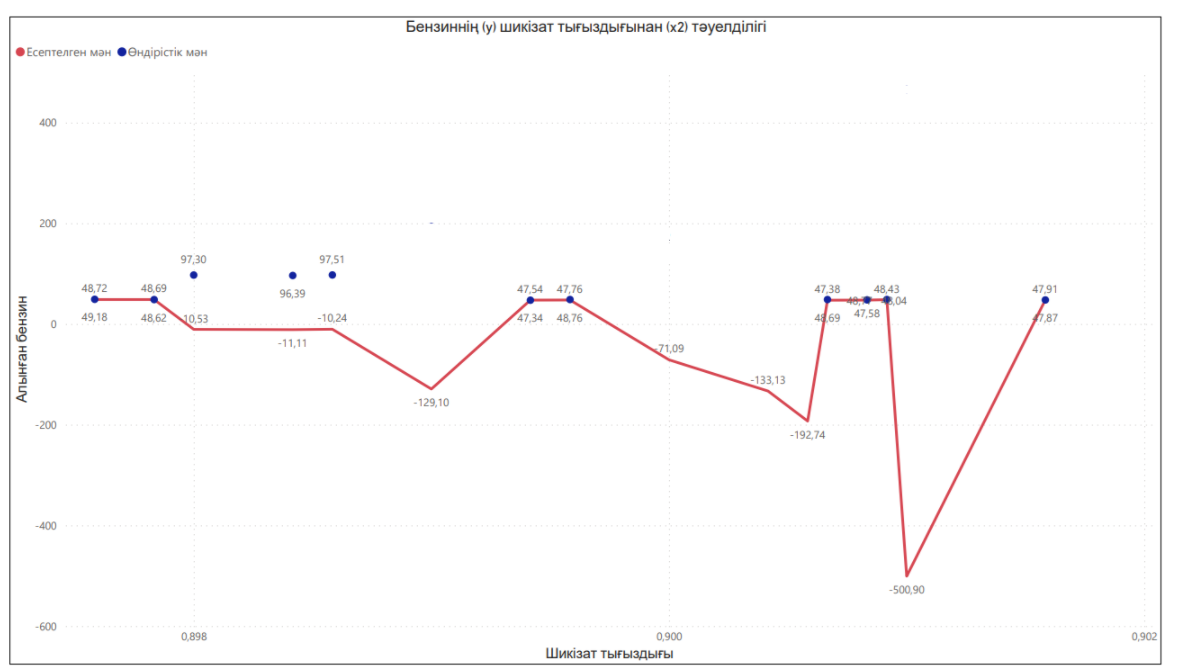
\includegraphics[width=0.8\textwidth]{media/ict/image95}
	\caption*{2-сурет. Бензин шығымының шикізат тығыздығынан тәуелділігі}
\end{figure}

\begin{equation*}
\begin{aligned}
c_0 &= -30.242; \quad c_1 = 0.161; \quad c_2 = -30.391; \\
c_3 &= -0.730; \quad c_4 = 0.185; \quad c_5 = -2.734; \quad c_6 = -0.004.
\end{aligned}
\end{equation*}

Осылайша, бензин шығысының параметрлерге айқын емес тәуелділігін
сипаттайтын теңдеу келесідей болады:

\begin{equation}
y=-30.342_0+0.161x_1-30.391x_2-0.730x_3+0.185x_4-2.734x_5-0.004x_6
\end{equation}

\begin{multicols}{2}
Тұрғызылған модельге сәйкес шикізат шығыны, катализатор, реактор мен
регенератордың температурасы, реактордағы қысым сияқты кіріс
параметрлеріне өнімнің шығысының (тұрақты бензин) графиктері алынды
(2-5-суреттер).

2-суретте бензин шығымының шикізат тығыздығына тәуелділік графигі
тұрғызылған. График бензин тығыздығының бензин шығымына кері
тәуелділігін көрсетеді.
\end{multicols}

\begin{figure}[H]
	\centering
	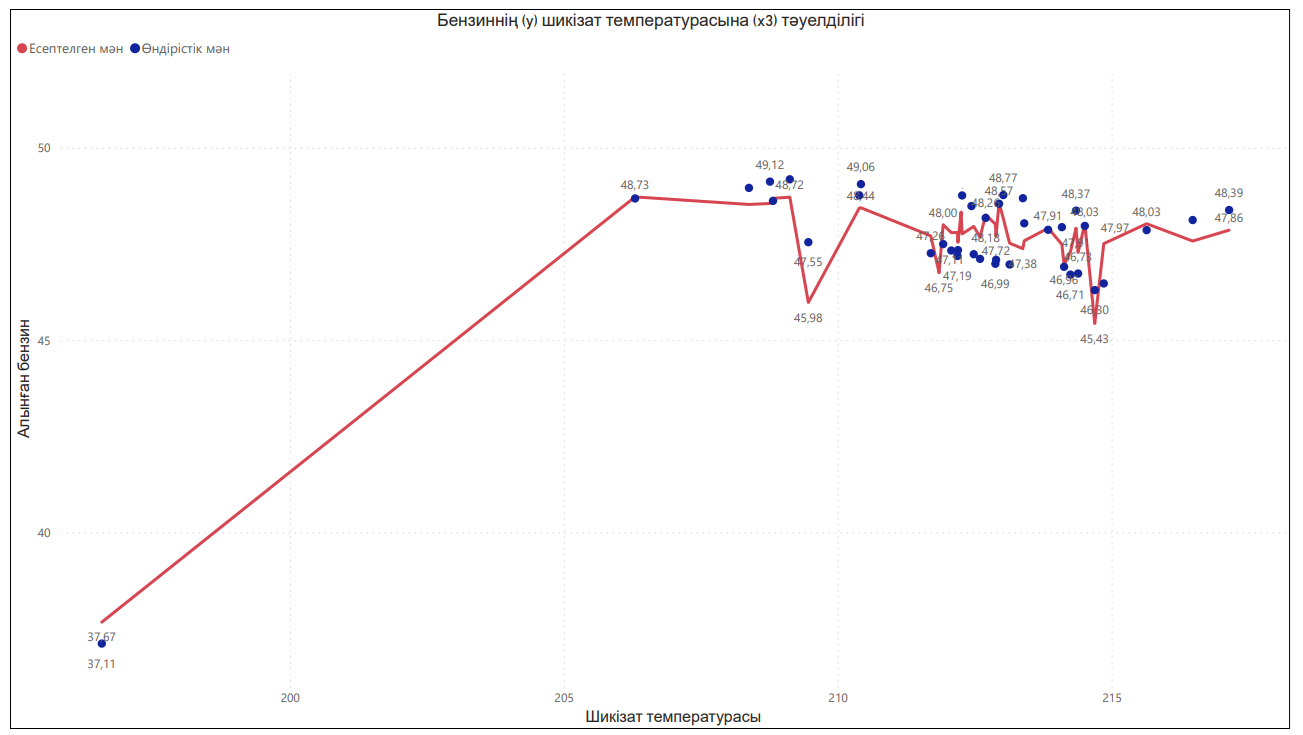
\includegraphics[width=0.8\textwidth]{media/ict/image96}
	\caption*{3-сурет. Бензин шығымының шикізат температурасынан тәуелділігі}
\end{figure}

\begin{multicols}{2}
3-суретте бензин шығымының шикізат температурасынан тәуелділігінің
өндірістік және есептелген мәндерінің сәйкестігін көруге болады. Шикізат
температурасын суретте көрсетілген мәнге дейін арттыру арқылы бензин
шығымын айтарлықтай көбейтуге болады. Сондай-ақ тұрғызылған графиктен
модель арқылы есептелген мәннің өндірістік мәндерге жақын болуы
модельдің адекваттылығын көрсетеді.
\end{multicols}

\begin{figure}[H]
	\centering
	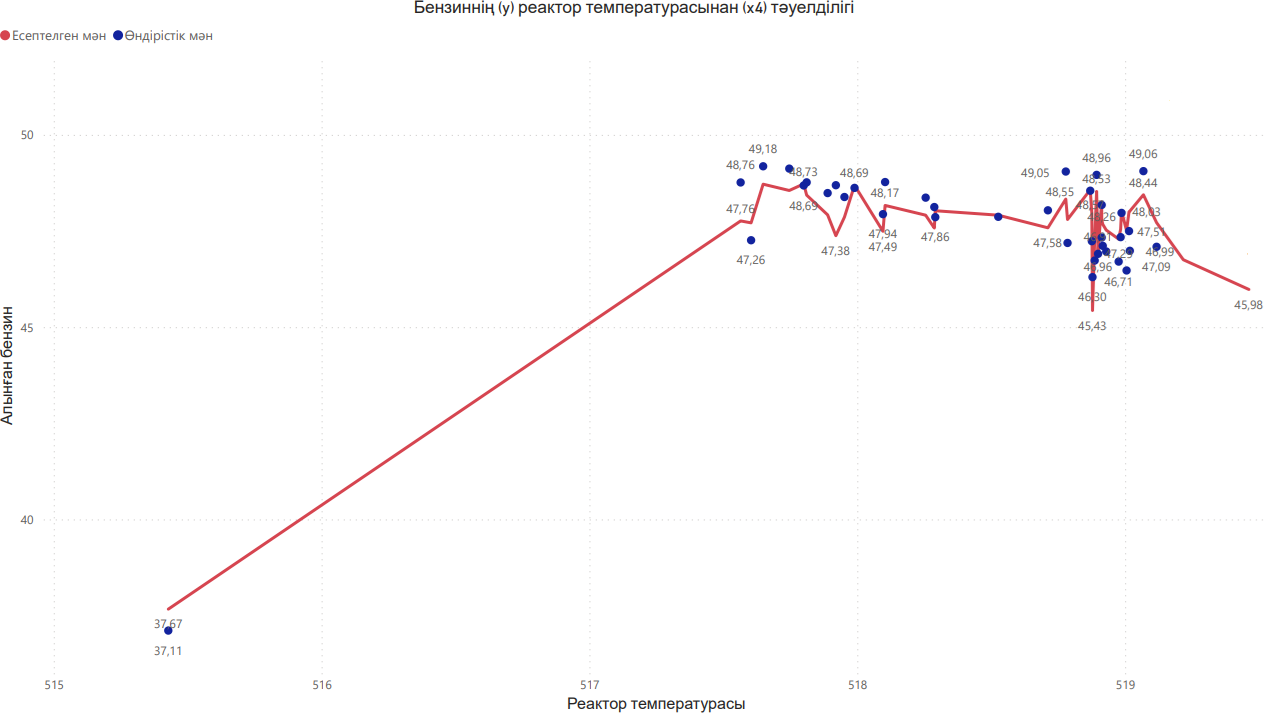
\includegraphics[width=0.8\textwidth]{media/ict/image97}
	\caption*{4 - сурет. Бензин шығымының реактор температурасынан
тәуелділігі}
\end{figure}

\begin{figure}[H]
	\centering
	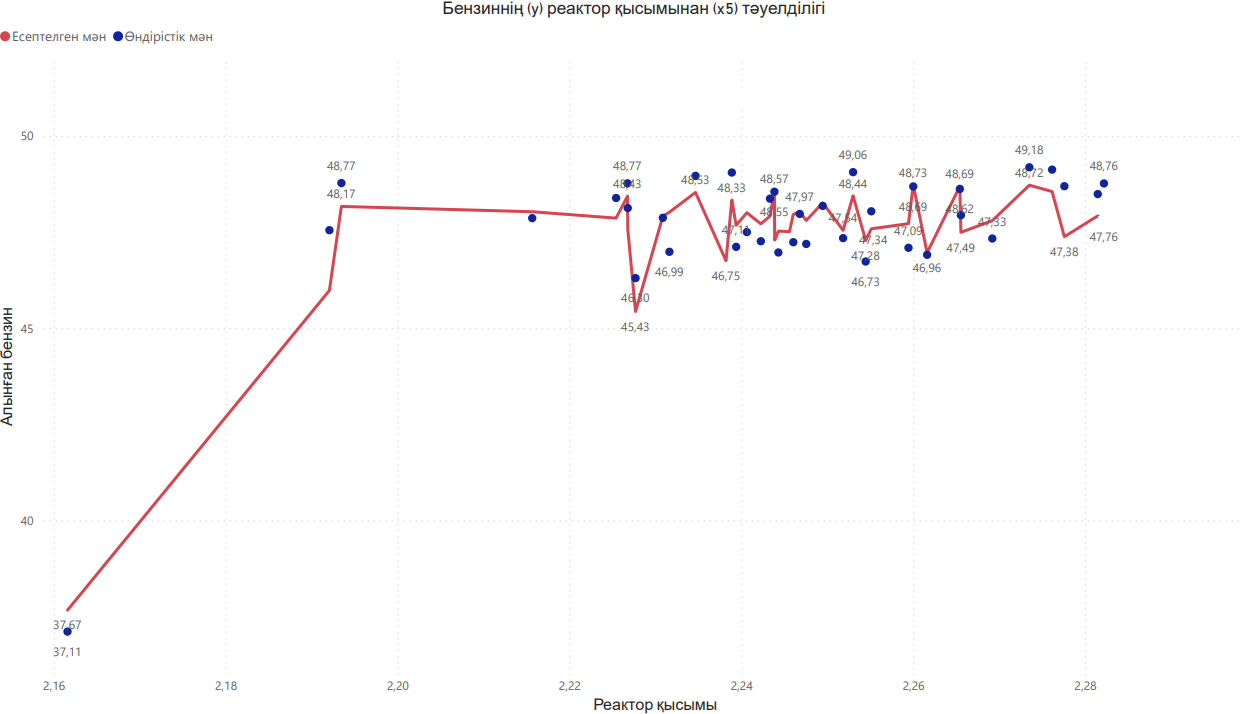
\includegraphics[width=0.8\textwidth]{media/ict/image98}
	\caption*{5-сурет. Бензин шығымының реактордағы қысымнан тәуелділігі}
\end{figure}

\begin{multicols}{2}
4,5-суреттерде бензин шығымының сәйкесінше реактор температурасы мен
қысымынан тәуелділік графигін көруге болады. Каталитикалық крекинг
бойынша негізгі процестер реактор бөлігінде жүргізілетіндіктен
реактордың параметрлерін есепке алу маңызды. Алынған графиктен
өндірістік және есептелген мәннің шамаларының жақындығын байқауға
болады.

Сынауға арналған деректер жиынтығындағы модельдің дәлдігін бағалау
орташа қалдық қате (MSE) 0.754-ке тең екенін көрсетті. Бұл мән болжанған
мәндердің нақты мәндерден ауытқуының рұқсат етілген деңгейін көрсетеді.
Детерминация коэффициенті (R2) 0.792-ге тең. R2 мәні модель тәуелді
айнымалының 79\% вариациясын көрсетеді, бұл көптеген әсер ететін
факторлары бар өнеркәсіптік процесс үшін жақсы нәтиже. Регрессия
коэффициенттері өнімнің шығуына әсер ететін ең маңызды факторлар мыналар
екенін көрсетті:

- реактордың температурасы: температураның жоғарылауы бензин сияқты
жеңіл өнімдердің шығуына оң әсер етеді;

- катализатордың сипаттамалары: катализатордың белсенділігі күткенге
сәйкес келетін бензин шығымымен тікелей корреляцияны көрсетті.

Регрессия моделі өзін өнімнің шығуын болжаудың сенімді құралы ретінде
көрсетті. Алайда, сызықтық емес тәуелділіктер немесе ескерілмеген
айнымалылар арасындағы өзара әрекеттесулер болған кезде оның дәлдігі
төмендеуі мүмкін. Болашақта болжамдардың дәлдігін жақсарту үшін гибридті
модельдерді қолдануды қарастырған жөн.

{\bfseries Қорытынды.} Бұл жұмыста Python бағдарламалық ортасында сызықтық
регрессия әдістерін қолдана отырып, каталитикалық крекинг қондырғысынан
өнімнің шығуын анықтау әдісі жасалды және бағаланды. Зерттеу нәтижелері
ұсынылған модельдің жоғары дәлдігін көрсетті, бұл оның өнеркәсіптік
тәжірибеде қолдану тиімділігін растайды. Регрессия моделін қолдану
өнімнің шығымына әсер ететін негізгі технологиялық параметрлерді
анықтауға және каталитикалық крекинг процесін оңтайландыруға мүмкіндік
берді. Детерминация коэффициентін (R2) және қалдық қателерді талдауды
қолдана отырып, модельдің сапасын бағалау болжамды мәндердің нақты
деректерге сәйкестігінің жоғары дәрежесін көрсетті. Осылайша, ұсынылған
тәсілді мұнай өңдеудегі технологиялық процестерді одан әрі оңтайландыру
үшін қолдануға болады, бұл каталитикалық крекинг қондырғыларының
өнімділігі мен тиімділігін арттырады. Болашақта болжамдардың дәлдігін
жақсарту үшін машиналық оқытудың күрделі әдістерін біріктіруге болады.
\end{multicols}

\begin{center}
{\bfseries Әдебиеттер}
\end{center}

\begin{references}

1. Han I.-S., Chung C.-B. Dynamic modeling and simulation of a fluidized
catalytic cracking process. Part II: Property estimation and
simulation // Chem. Eng. Sci. -2022. -Vol. 56. -P. 1973-1990.
\href{https://doi.org/10.1016/S0009-2509(00)00494-2}{DOI
10.1016/S0009-2509(00)00494-2}

2. Emberru R.E., Patel R., Mujtaba I.M., John Y.M. A Review of Catalyst
Modification and Process Factors in the Production of Light Olefins
from Direct Crude Oil Catalytic Cracking // Chemical Engineering,
Faculty of Engineering \& Digital Technologies. -2024. --Vol. 6(11).
DOI 10.3390/sci6010011

3. Palos R., Rodríguez, E., Gutiérrez A., Bilbao J., \& Arandes, J. M.
Kinetic modeling for the catalytic cracking of tires pyrolysis oil //
Fuel. -2022. -Vol. 309.
\href{https://doi.org/10.1016/j.fuel.2021.122055}{DOI
10.1016/j.fuel.2021.122055}

4. Orazbayev B.B., Shangitova Z.Y., Orazbayeva K.N., Serimbetov B.A.,
Shagayeva A.B. Studying the Dependence of the Performance Efficiency
of a Claus Reactor on Technological Factors with the Quality
Evaluation of Sulfur on the Basis of Fuzzy Information //Theor. Found.
Chem. Eng., -2020.-Vol. 54. - P. 1235--1241. DOI
\\10.1134/S0040579520060093

5. Taşkin H., Kubat C., Uygun Ö., Arslankaya S. FUZZYFCC: Fuzzy logic
control of a fluid catalytic cracking unit (FCCU) to improve dynamic
performance // Computers \& chemical engineering. -2006. - Vol. 30(5).
- P. 850-863. \href{https://doi.org/10.1016/j.compchemeng.2005.12.016}{DOI
10.1016/j.compchemeng.2005.12.016}

6. Precup R.E., Nguyen A.T., Blažič S. A survey on fuzzy control for
mechatronics applications //International Journal of Systems Science.-
2024.- Vol.55(4).-P. 771-813. DOI \href{https://doi.org/10.1080/00207721.2023.2293486}{10.1080/00207721.2023.2293486}


7. Hе G., Zhou C., Luo T., Zhou L., Dai Y., Dang, Y., Ji, X. Online
optimization of Fluid Catalytic Cracking process via a Hybrid model
based on Simplified structure-Oriented Lumping and case-based
reasoning // Industrial \& Engineering Chemistry Research. -2020.-Vol.
60(1). - P. 412-424. DOI
\href{http://dx.doi.org/10.1021/acs.iecr.0c04109}{10.1021/acs.iecr.0c04109}

8. Beatriz Flamia Azevedo, Ana Maria A.C. Rocha, Ana I. Pereira Hybrid
approaches to~optimization and~machine learning methods: a~systematic
literature review. Machine Learning. -2024. -Vol 113. - P. 4055 -
4097. DOI \\\href{http://dx.doi.org/10.1007/s10994-023-06467-x}{10.1007/s10994-023-06467-x}

9.Orazbayev B.B., Kenzhebayeva S.T., Orazbayeva K. N. Development of
Mathematical Models and Modelling of Chemical Technological Systems
using Fuzzy-Output Systems//Applied Mathematics \& Information Sciences
-2019. -Vol. 13(4).-P.653-664.DOI 10.18576/amis/130417

10.Yang F., Xu M., Lei W., Lv J. Artificial intelligence methods applied
to catalytic cracking processes//Big Data Mining and
Analytics.-2023.-Vol. 6(3).-P. 361-380. DOI \href{http://dx.doi.org/10.26599/BDMA.2023.9020002}{10.26599/BDMA.2023.9020002}

11.Santander V. Kuppuraj, C.A. Harrison, M. Baldea An open source FCC
model to support developing and bench-marking process control and
operations strategies // Computers \& Chemical Engineering. -2022. -Vol.
164. DOI \\\href{https://doi.org/10.1016/j.compchemeng.2022.107900}{10.1016/j.compchemeng.2022.107900}

12.Josiah P.N., Otaraku I.J., Evbuomwan B.O. Servo and Regulatory
Response of an Industrial Fluid Catalytic Cracking (FCC) Unit under
Fuzzy Logic Supervisory Control // Eng. Technol. J. -2023. -Vol.41. -P.
1139-1151. DOI 10.30684/etj.2023.139485.1432

13.Orazbayev B., Boranbayeva N., Makhatova V., Rzayeva L., OspanovY.,
Kurmashev I., Kurmangaziyeva L. Devel-opment and Synthesis of Linguistic
Models for Catalytic Cracking Unit in a Fuzzy Environment. Processes.
-2024. -Vol. 12(8). DOI
\href{https://doi.org/10.3390/pr12081543}{10.3390/pr12081543}

14. Oloruntoba A., Zhang Y., Hsu C.S. State-of-the-Art Review of Fluid
Catalytic Cracking (FCC) Catalyst Regen-eration Intensification
Technologies//Energies.-2022.-Vol.15.
DOI 10.3390/en15062061

15.Letzsch W. Fluid Catalytic Cracking (FCC) in Petroleum Refining. In:
Treese, S., Pujadó, P., Jones, D. (eds) Handbook of Petroleum Processing
// Springer, Cham. -2015. DOI10.1007/978-3-319-14529-7\_2

16.Amblard, B., Singh R., Gbordzoe E., Raynal L.CFD modeling of the coke
combustion in an industrial FCC regenerator // Chemical Engineering
Science.- 2016. - P. 731- 742.
DOI
\href{http://dx.doi.org/10.1016/j.ces.2016.12.055}{10.1016/j.ces.2016.12.055}

17. Idris M., Burn A. CFD Modelling Gas-Solid Flows in CFB // FCC Riser
Reactors: Simulation Using Kinetic Theory of Granular Flow (KTGF) in a
Fully Developed Flow Situation. -American institute of chemical
engineers, 2008. 1-19

18. Barbosa et.al., A. C., Three-Dimensional Simulation of Catalytic
Cracking Reactions in an Industrial Scale Riser Using a 11-lump Kinetic
Model. Chem. Eng. Trans. -2013.- 32. -P. 637-642 DOI
\href{http://dx.doi.org/10.3303/ACOS1311004}{10.3303/ACOS1311004}

19. Sabzi H.Z. Developing an intelligent expert system for streamflow
prediction, integrated in a dynamic decision support system for managing
multiple reservoirs: a case study // Expert systems with applications.
-2017. -Vol. 82. -№3. -C.145--163. DOI 10.1016/j.eswa.2017.04.039
\end{references}

\begin{authorinfo}
\hspace{1em}\emph{{\bfseries Авторлар туралы мәліметтер}}

Боранбаева Н.Б. -- докторант, Л.Н.Гумилев атындағы Еуразия Ұлттық
университеті, сеньор лектор, Astana IT University, Астана, Қазақстан,
e-mail: ades\_98@mail.ru;

Оразбаев Б.Б.- профессор, т.ғ.д., Л.Н.Гумилев атындағы Еуразия Ұлттық
университеті, Астана, Қазақстан, e-mail: \\batyr\_o@mail.ru;

Рзаева Л.Г.- қауымдастырылған профессор, Astana IT University, Астана,
Қазақстан, e-mail:
\href{mailto:l.rzayeva@astanait.edu.kz}{\nolinkurl{l.rzayeva@astanait.edu.kz}};

Карабаев Ж.А. -PhD, аға оқытушы, М.Әуезов атындағы Оңтүстік Қазақстан
университеті, Шымкент, Қазақстан,\\ e-mail:jalal45@mail.ru

Серимбетов Б.А.- техникалық ғылымдар кандидаты, қауымдастырылған
профессор, Қ.Құлажанов атындағы Қазақ технология және бизнес
университеті ,Астана, Қазастан, e-mail:
\href{mailto:sba_rnmc@mail.ru}{\nolinkurl{sba\_rnmc@mail.ru}}.

\hspace{1em}\emph{{\bfseries Information about the authors}}

Boranbayeva N.- doctoral student at L. N. Gumilyov Eurasian National
University, senior lecturer, Astana IT University, Astana, Kazakhstan,
e-mail: ades\_98@mail.ru;

Orazbayev B.- Doctor of Technical Sciences, Professor, L.N.Gumilyov
Eurasian National University, Astana, Kazakhstan, e-mail:
batyr\_o@mail.ru;

Rzayeva L.- Associate Professor, Astana IT University, Astana,
Kazakhsta, e-mail:
\href{mailto:l.rzayeva@astanait.edu.kz}{\nolinkurl{l.rzayeva@astanait.edu.kz}};

Karabayev Zh.- PhD, senior lecturer, Mukhtar Ayezov South Kazakhstan
University, Shymkent, Kazakhstan, \\e-mail:
\href{mailto:jalal45@mail.ru}{\nolinkurl{jalal45@mail.ru}}.

Serimbetov B.- Candidate of Technical Sciences, associate
Professor,K.Kulazhanov Kazakh University of Technology and Business,
Astana, Kazakhstan, e-mail:
\href{mailto:sba_rnmc@mail.ru}{\nolinkurl{sba\_rnmc@mail.ru}}.
\end{authorinfo}
